\begin{frame}{one connection, multiple requests}
    \begin{itemize}
    \item HTTP/0.9, HTTP/1.0 --- one request+response per connection
        \begin{itemize}
        \item big efficiency problem
        \end{itemize}
    \item solution 1: persistent connections
    \item solution 2: pipelining
    \item solution 3 (HTTP/2+): multiple `streams' in one connection
    \end{itemize}
\end{frame}

\begin{frame}{end-of-request/response}
    \begin{itemize}
    \item body of request/response can be variable length
    \vspace{.5cm}
    \item so when does request/response end if it has a body?
    \item HTTP/1.0 original solution (RFC 1945)
        \begin{itemize}
        \item ``the length of that body may be determined in two ways. If a Content-Length field is present, the value in bytes represents the length of the Entity-Body. Otherwise, the body length is determined by the closing of the connection by the server.''
        \end{itemize}
    \item advantage of latter idea: don't need to generate whole document before sending headers
    \item disadvantage: no persistent connections!
    \end{itemize}
\end{frame}


\providecommand{\chunksize}[1]{\textbf{\color{violet!80}#1}}
\begin{frame}[fragile,label=chunked]{chunked transfer coding}
\begin{Verbatim}[commandchars=\\\{\}]
HTTP/1.1 200 OK
Content-Type: text/plain
\textbf{Transfer-Coding: chunked}
...

\chunksize{1B}
\textbf{This is 0x1B bytes of text.}
\chunksize{21}
\textbf{And 0x21 bytes}
\textbf{with more lines.}
\chunksize{0}
\end{Verbatim}
\end{frame}

\begin{frame}{pipelining}
\begin{tikzpicture}
\tikzset{
    nodeline/.style={draw,ultra thick},
    msgline/.style={draw,very thick,-Latex},
    msgbox/.style={draw,fill=white,font=\small\tt,align=left},
}
\draw[nodeline] (0, -.5) -- ++(0, -7) node[pos=0,above] {client};
\draw[nodeline] (12, -.5) -- ++(0, -7) node[pos=0,above] {server};
\draw[msgline] (0, -1) -- (12, -2) node[midway,msgbox] {
    GET /image1.png HTTP/1.1
    \ldots
};
\draw[msgline] (0, -1.5) -- (12, -2.5) node[midway,msgbox] {
    GET /image2.png HTTP/1.1
    \ldots
};
\draw[msgline] (0, -2) -- (12, -3) node[midway,msgbox] {
    GET /script.js HTTP/1.1
    \ldots
};
\draw[msgline] (12, -2.5) -- (0, -3) node[midway,below,msgbox] {
    HTTP/1.1 200 OK
    \ldots
};
\draw[msgline] (12, -4) -- (0, -5) node[midway,msgbox] {
    HTTP/1.1 200 OK
    \ldots
};
\draw[msgline] (12, -5) -- (0, -6) node[midway,msgbox] {
    HTTP/1.1 200 OK
    \ldots
};
\end{tikzpicture}
\end{frame}

\begin{frame}{HTTP/1.1 `pipelining'}
    \begin{itemize}
    \item send series of requests before receiving any response
    \item potentailly server can potentially process requests in parallel
    \vspace{.5cm}
    \item need to handle resending requests if connection dropped early
    \end{itemize}
\end{frame}

\begin{frame}{HTTP/2.0 multiple streams}
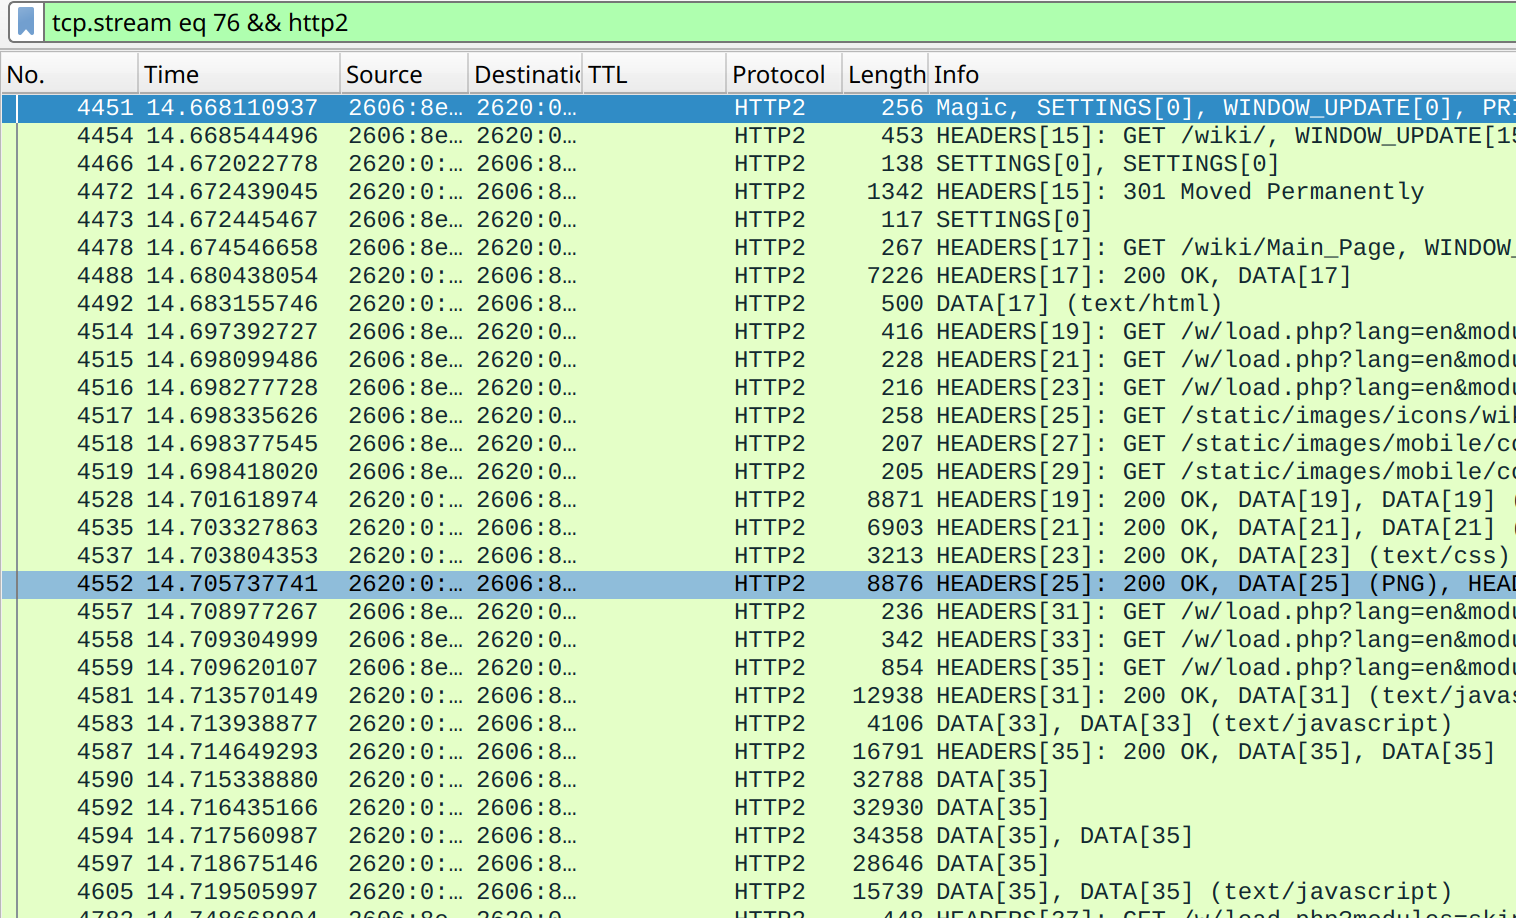
\includegraphics[width=\textwidth]{../http/http2-multi-reqres}
\end{frame}
